\documentclass{caosp308}
\usepackage{graphicx}
\usepackage{natbib}
\usepackage{amsmath}
\usepackage{amsfonts}
\usepackage{amssymb}
\bibliographystyle{caosp308}
\articleNo{300}
\pubyear{2020}
\volume{50}
\volnumber{4}
\firstpage{1}
\received{July 9, 2020}
\accepted{October 11, 2020}

\def\BibTeX{{\rm B\kern-.05em{\sc i\kern-.025em b}\kern-.08em
             T\kern-.1667em\lower.7ex\hbox{E}\kern-.125emX}}

\begin{document}

\hauthor{M.V.\, Vavrukh and D.V.\, Dzikovskyi}
\htitle{Exact solution for the rotating polytropes with index unity}
\title{Exact solution for the rotating polytropes with index unity, its approximations and some applications}

\author{
		M.V.\, Vavrukh\orcid{0000-0003-2129-5867} and 
		D.V.\, Dzikovskyi\orcid{0000-0002-9607-7787}
		}

\institute{Department of Astrophysics, Ivan Franko National University,
            Kyrylo \& Methodiy str. 8, 79005 Lviv, Ukraine, \email{mvavrukh@gmail.com}}

\date{July 9, 2020}
\maketitle
\begin{abstract}
The fundamental stages of development of the polytropic theory of stars with axial rotation are considered as a generalization of the Lane-Emden theory. The solution of the differential equilibrium equation for the polytropic star model with index $n=1$ and axial rotation with the angular velocity $\omega$ is presented in the form of infinite series of the Legendre polynomials and the spherical Bessel functions. Two variants of the approximate solution in the form of the finite number of terms are proposed. Integration constants were found in a self-consistent way using the integral form of the equilibrium equation and the iteration numerical method. Dependence of the geometrical and physical characteristics of the model on the dimensionless angular velocity $\Omega=\omega(2\pi G\rho_{\rm c})^{-1/2}$ (where $\rho_{\rm c}$ is the density in the centre) is analyzed. A comparison with the results of other authors is performed. The obtained critical value of the angular velocity $\Omega_{\rm max}$, when an instability occurs  is smaller than in other works  \citep[and et al.]{1933MNRAS..93..390C,1964ApJ...140..552J}. The inverse problem is also considered -- a determination of the polytropic model parameters for individual stars based on the solution of the equilibrium equation according to the values of their masses and radii, which are known from observations. In particular, the model parameters for the star $\alpha$ Eri, as well as a similar ``class'' of the star models of types O5$\div$G0, were determined. The solution of the equilibrium equation for the polytrope $n=1+\delta$ (where $\delta$ is a small value) is obtained using the method of perturbation theory.

\keywords{stars: rotation -- stars: interiors -- stars: fundamental parameters -- stars: statistics.}\\
{\bf PACS} number(s): 97.20.-w
\end{abstract}

%
%__________________________________________________________________________________

\section{Introduction}
\label{sect_01da}
The principles of the polytropic theory of solar-like stars were created by the works of  \citet{1870AmJS...50...57L}, \citet{1907gask.book.....E}, \citet{1930MNRAS..91...63F}, \citet{1926ics..book.....E} and other researchers in the first half of the last century. This theory is based on the equilibrium equation of a star with the polytropic equation of state
\begin{equation}
\label{eq_001da}
P ({\bf r})\:=K\rho^{1+1/n} ({\bf r}),
\end{equation}
where $P ({\bf r})$ is the pressure at the radius-vector ${\bf r}$,  $\rho({\bf r})$ is the local density of matter, and $K$ and $n$ are  constants. It yields a determination of main relations between the polytrope characteristics and describes stability of stars. An idea of the polytropic dependence between the pressure and density is successfully used for a construction of the cold degenerate dwarfs theory \citep{1931ApJ....74...81C}.

The axial rotation is a factor that is common for various celestial objects -- the stars of main sequence, pulsars, white dwarfs and black holes. The equilibrium equation of polytrope without rotation with spherical symmetry of matter distribution is an ordinary differential equation of the second order, which is known as the Lane-Emden-Fowler equation. The equilibrium equation for the polytropic model with axial rotation in a general case (for an arbitrary value of the index $n$) is a non-linear differential equation of second order in partial derivatives. The exact solution of the equation is known only for the particular case $n=0$, from which the Maclaurin formula  is obtained \citep[see][]{1969efe..book.....C} that determines the relations between the angular velocity and eccentricity of a rotating homogeneous ellipsoid.

To evaluate the influence of rotation on the Sun's characteristics, \citet{1923MNRAS..83..118M} found an approximate solution of the equilibrium equation for $n=3$ for the case of a small angular velocity, by linearizing the equation. Such approximation corresponds to the first order of perturbation theory. Using the method of  \citet{1923MNRAS..83..118M}, \citet{1933MNRAS..93..390C} obtained the solutions with the help of a numerical integration for the polytropes with indices $n=1.0, 1.5, 2.0, 2.5, 3.0$. \citet{1937ZA.....14..135K} pointed out that in the particular case of $n=1$ with an axial symmetry  the equilibrium equation allows for a separation of variables. He found a set of fundamental solutions in the form of products of the Legendre polynomials and the spherical Bessel function of the first kind. However, the question of finding a general solution, by the given boundary conditions, Kopal did not consider.

\citet{1964ApJ...140..552J} went beyond a small rotational velocity approximation. He found an approximate solution for the polytropes with indices $n=1.0, 1.5, 2.0,\newline 2.5, 3.0$ and calculated dependence of the polytrope characteristics on the angular velocity in the interval $0\leq\omega\leq\omega_{max}(n)$. Unfortunately, the solutions were not presented in the publication, which makes it impossible to analyze their dependence on the angular velocity as well as to use the solutions for the calculation of other characteristics.

In the work of \citet*{1965MNRAS.131...13M} there is generalized the Milne -- Chandrasekhar approach by a more accurate description of the outer polytrope region. Aiming to find integration constants \citep{1923MNRAS..83..118M,1933MNRAS..93..390C} and also to determine the fitting parameters \citep*{1965MNRAS.131...13M}, the authors applied the traditional in the stellar surface theory approximation, which is based on the usage of the general multipole form of potential, created by an unknown distribution of matter in the inner part of the star. The common characteristic of these works is the first approximation relative to rotation influence. Therefore integration constants and fitting parameters do not depend on the angular velocity, but only on the polytropic index \citep*{1923MNRAS..83..118M,1933MNRAS..93..390C,1965MNRAS.131...13M}. The partial solution of the equilibrium equation which is considered by \citet{1980Ap&SS..71..415C} at $n=1$,  improves Chandrasekhar's solution \citep{1933MNRAS..93..390C} by the determination of  integration constants numerically.

In spite of the long research history, the problem of the calculation of characteristics of the polytropic model remains relevant and has both methodological and applied importance. It should be mentioned recent works of \citet{2015MNRAS.448..456K} and \citet{2017MNRAS.467.4965K}, in which the computer methods were used to calculate the characteristics of individual stars based on the polytropic model at $n=1$. The polytrope model is a good zero approximation for the calculation of the characteristics of massive dwarfs \citep{1964ApJ...140..552J,2010JPS.14...4901V}. It can be used to describe neutron stars, circumstellar disks, gas giant planets, and in the theory of stability and pulsation of stars.

In the work of  \citet{2019MMC.6...153V} it is shown that the finding of the solutions of the equilibrium equation for the polytropes with rotation more accurately requires the usage of a multi-component expansion for the Legendre polynomials. In this case the correct definition of integration constants is provided by the integral form of the equilibrium equation, which is equivalent to the explicit calculation of gravitational potential at some point of polytrope by the known solution of the equilibrium equation.

The model with $n=1$ plays the role of the standard in the polytropic theory. Finding a solution of a linear inhomogeneous differential equation of the second order with partial derivatives is a simpler problem than finding solutions of a non-linear equation at $n>1$. Therefore, with polytrope with $n=1$ there  is tested a new method of finding the equilibrium equation solutions, which can be generalized later for the model with an arbitrary $n$. The problem of calculation of the polytropic characteristics with $n=1$ has independent meaning, as an example of the problem that allows for solutions with high precision. The maximal value of the angular velocity for this model is quite large ($\Omega_{\rm \max}=0.245$), therefore it is suitable for the calculation of the characteristics of the individual observed stars with rapid axial rotation.

The purpose of our work is to obtain the correct analytical approximation of the solution of the equilibrium equation for the polytrope with $n=1$ and solid-body rotation. In this way we simultaneously use differential and integral forms of the equilibrium equation (section~\ref{sect_02da}). Two representations of the solution of the differential equation in the form of the infinite series, as well as two basic approximations in the form of the finite number of terms, are shown in section~\ref{sect_03da}. The self-consistent method of the calculations of integration constants based on the integral equation is described in section~\ref{sect_04da}. The results of calculations of the polytrope characteristics dependence and integration constants on the angular velocity are shown in section~\ref{sect_05da}. In section~\ref{sect_06da} it is shown the way how the solution of the equilibrium equation of the polytrope with $n=1$ can be used to find an approximate solution at $n=1+\delta$, where $\delta$ is a small value. The application of the found basic approximations and their linear combinations is considered in section~\ref{sect_07da}, where the polytropic model is built for the star $\alpha$ Eri and models for the stars of classes O5$\div$G0.

%________________________________________________________________________________________

\section{The two forms of the equilibrium equation}
\label{sect_02da}

In the presence of rotation the hydrostatic equilibrium equation is rewritten in the non-inertial (rotating) coordinate system in the form \citep{1933MNRAS..93..390C}
\begin{equation}
\label{eq_002da}
\nabla P({\bf r})=-\rho({\bf r})\left\{\nabla\Phi_{\rm grav}({\bf r})+\nabla\Phi_{\rm c}({\bf r})\right\},
\end{equation}
where
\begin{equation}
\label{eq_003da}
\Phi_{\rm grav}({\bf r})\:=\:-G\int\frac{d{\bf r}^{'}\rho({\bf r}^{'})}{|{\bf r}-{\bf r}^{'}|}
\end{equation}
is the gravitational potential inside the star and $\Phi_{\rm c}({\bf r})$ is the centrifugal potential. If the axis $Oz$ of the spherical coordinate system coincides with the axis of rotation, then
\begin{equation}
\label{eq_004da}
\Phi_{\rm c}({\bf r})\:=\:-\frac12\:\omega^2 r^2\sin^2\theta.
\end{equation}
Here $\theta$ is the polar angle and $\omega$ is the angular velocity of reference frame, which is considered as constant.

Substituting the expressions \eqref{eq_001da} for $n=1$, \eqref{eq_003da} and \eqref{eq_004da} in Eq.~\eqref{eq_002da} and taking the divergence, the equilibrium equation is obtained in the form of the differential equation that determines the density distribution,
\begin{equation}
\label{eq_005da}
2K\Delta\rho({\bf r})=-4\pi G\rho({\bf r})+\frac{1}{2}\omega^2\Delta(r^2\sin^2\theta).
\end{equation}
In the presence of axial symmetry  $(\rho({\bf r})=\rho(r,\theta))$ the Laplace operator is written in the form
\begin{eqnarray}
\label{eq_006da}
\begin{split}
&\Delta=\Delta_r +\frac{1}{r^2}\:\Delta_{\theta},\,
\Delta_r=\frac{1}{r^2}\frac{\partial}{\partial r}\:\left(r^2 \frac{\partial}{\partial r}\right),\\
&\Delta_{\theta}=\frac{\partial}{\partial t}\:(1-t^2)\:\frac{\partial}{\partial t},
\end{split}
\end{eqnarray}
at $t=\cos \theta$, therefore $\Delta\:(r^2 \sin^2 \theta)=4$. Introducing the dimensionless radial coordinate $\xi = r/\lambda$, as well as using the substitution
\begin{equation}
\label{eq_007da}
\rho(r,\theta)\:=\:\rho_{\rm c} \:Y(\xi,\theta),
\end{equation}
where $\rho_{\rm c}$ is the density of matter in the stellar centre, we transform Eq.~\eqref{eq_005da} to the dimensionless form
\begin{equation}
\label{eq_008da}
\Delta_{\xi,\theta}\:Y(\xi,\theta)\:=\:\Omega^2-Y(\xi,\theta).
\end{equation}
Herewith the scale  $\lambda_n$, the dimensionless angular velocity $\Omega$ and the Laplacian operator are determined by the relations
\begin{eqnarray}
\label{eq_009da}
\begin{split}
&\lambda=\left(\frac{K}{2\pi G}\right)^{1/2},\,\,\Omega=\frac{\omega}{(2\pi G\rho_{\rm c})^{1/2}},\\
&\Delta_{\xi,\theta} = \Delta_{\xi} +\frac{1}{\xi^2}\:\Delta_{\theta}, \, \Delta_{\xi} =\frac{1}{\xi^2}\frac{\partial}{\partial\xi} \left(\xi^2 \frac{\partial}{\partial\xi}\right).
\end{split}
\end{eqnarray}
According to definition \eqref{eq_007da}, $Y(0,\theta)=1$ and the condition $\partial Y(\xi,\theta)/\partial\xi=0$ at $\xi=0$ corresponds to the solutions regular in the vicinity of $\xi=0$. At large values of $\Omega$  the non-monotonous dependence  $Y (\xi,\theta)$  on the variable $\xi$ in the equator region, as well as the leakage of matter, are possible. The stability conditions of stars in the equatorial region
\begin{equation}
\label{eq_010da}
Y \left(\xi,\:\frac{\pi}{2}\right)\:=\:0, \quad \frac{\partial}{\partial\xi}\:Y \left(\xi,\:\frac{\pi}{2}\right)\:=\:0
\end{equation}
determine the maximal permissible value of the parameter $\Omega_{\rm max}$ and the corresponding value of the equatorial radius $\xi_e^{\rm max}$. According to definition \eqref{eq_007da}, only positive solutions of  Eq.~\eqref{eq_008da} have a physical meaning, which is the two-dimensional differential equation of the second order in partial derivatives with a dimensionless parameter $\Omega\geq 0$.

Eq.~\eqref{eq_008da} is similar to the Poisson equation, therefore it can formally be considered as the equation for dimensionless gravitational potential, which is created by the dimensionless density distribution $(4\pi)^{-1}\cdot\{\Omega^2 - Y (\xi,\theta)\}$.
In this regard, this equation can be rewritten in the integral form
\begin{equation}
\label{eq_011da}
Y (\xi,\theta) = 1+\sum\limits^{\infty}_{l=1} C_{2l}\:\xi^{2l} P_{2l}(t)-\frac{1}{4\pi}\int
\bigl\{\Omega^2-Y(\xi^{'},\theta^{'})\bigr\}\:Q ({\boldsymbol\xi},{\boldsymbol\xi}^{'})\:d{\boldsymbol\xi}^{'},
\end{equation}
where $C_{2l}$ are integration constants,  $P_{2l}(t)$ are the Legendre polynomials of the $2l$-th order, the kernel of the equation is
\begin{equation}
\label{eq_012da}
Q ({\boldsymbol\xi},{\boldsymbol\xi}^{'}) = |{\boldsymbol\xi}-{\boldsymbol\xi}^{'}|^{-1} - ({\xi}^{'})^{-1},
\end{equation}
and the integration is performed over the stellar volume. Taking into account the identity
\begin{equation}
\label{eq_013da}
\Delta_{\xi,\theta}\:\{\xi^l\:P_l (t) \}\:=\:0,
\end{equation}
it is easy to verify that Eqs.~\eqref{eq_008da} and \eqref{eq_011da} are equivalent.

The gravitational potential inside a star \eqref{eq_003da} is related to dimensionless potential
\begin{equation}
\label{eq_014da}
\Phi({\boldsymbol\xi})\:=\:-\frac{1}{4\pi}\:\int \frac{Y({\boldsymbol\xi}^{'})}{|{\boldsymbol\xi} -{\boldsymbol\xi}^{'}|}\:d{\boldsymbol\xi}^{'}
\end{equation}
as follows
\begin{equation}
\label{eq_015da}
\Phi_{\rm grav} ({\bf r})\:=\:4\pi\:G\:\lambda^2 \rho_{\rm c}\:\Phi({\boldsymbol\xi}).
\end{equation}
Rewriting Eq.~\eqref{eq_002da} in dimensionless variables, we obtain the relation
\begin{equation}
\label{eq_016da}
\frac{\partial}{\partial\xi}\:\biggl\{\Phi_n (\xi,\theta) + Y (\xi,\theta)\biggr\} \:=\:
\frac{\Omega^2}{3}\:\xi\:\biggl\{1-P_2 (t) \biggr\}.
\end{equation}
Eq.~\eqref{eq_011da} can be represented in terms $Y (\xi,\theta)$, $\Phi_n (\xi,\theta)$, namely
\begin{eqnarray}
\label{eq_017da}
Y (\xi,\theta)\!+\!\{\Phi(\xi,\theta)-\Phi(0,0)\}
\!=\!1\!+\!\sum_{l=1}\!C_{2l} \xi^{2l}\!P_{2l} (t)\!+\!\Omega^2 \bigl\{\Phi_0 (\xi,\theta)\!-\!\Phi_0 (0,0) \bigr\},
\end{eqnarray}
where $\Phi_0 (\xi,\theta)$ determines expression \eqref{eq_014da} at $Y({\boldsymbol\xi}^{'})\equiv1$. This allows us to convert Eq.~\eqref{eq_016da} to a form
\begin{eqnarray}
\label{eq_018da}
\frac{\partial}{\partial\xi}\!\left\{\sum_{l=1} C_{2l}\:\xi^{2l}\:P_{2l} (t) + \Omega^2\:[\Phi_0 (\xi,\theta)-\Phi_0 (0,0)]\right\}
=\xi\:\frac{\Omega^2}{3}\:\biggl(1\:-\:P_2 (t)\biggr).
\end{eqnarray}
The difference of potentials $\Phi_0 (\xi,\theta)-\Phi_0 (0,0)$ is easy to calculate using an expansion in the series of kernel $Q ({\boldsymbol\xi},{\boldsymbol\xi}^{'})$ for the Legendre polynomials and performing integration over the variable $0\leq\xi'\leq\xi_0(t)$, where $\xi_0(t)$ is the root of the equation $Y(\xi,\theta)=0$. It determines the equation of the polytrope surface. In this way we find that
\begin{eqnarray}
\label{eq_019da}
\begin{split}
&\Phi_0 (\xi,\theta)-\Phi_0 (0,0)=-\frac{1}{4\pi}\int d{\boldsymbol\xi}^{'}Q({\boldsymbol\xi}, {\boldsymbol\xi}^{'})
=\frac{\xi^2}{6}+\frac{\xi^2}{2}\:P_2(t)I_2+\sum\limits_{l=2}^\infty\xi^{2l}P_{2l}(t)I_{2l},\\
&I_2=-\int\limits_{-1}^{1}P_2(t')\ln\xi_{0}(t')dt',\,
I_{2l}=\frac{1}{4}(l-1)^{-1}\int\limits_{-1}^{1}P_{2l}(t')(\xi_0(t'))^{2-2l)}\,dt'\,\,\,\text{at}\,\,\,l\geq2.
\end{split}
\end{eqnarray}
We note that $I_{2l}=0$ at $l\geq2$, where the star is approximated by the rotational ellipsoid \citep{1969efe..book.....C}. Substituting expression \eqref{eq_019da} into Eq.~\eqref{eq_018da}, we get the equality
\begin{equation}
\label{eq_020da}
(2C_2+\Omega^2I_2)P_2(t)+\sum\limits_{l=2}^\infty(C_{2l}+\Omega^2I_{2l})2l\xi^{2l-2}P_{2l}(t)=-\frac{\Omega^2}{3}P_{2}(t).
\end{equation}
Given the orthogonality of the Legendre polynomials, it follows that
\begin{equation}
\label{eq_021da}
C_2=-\frac{\Omega^2}{6}\biggl(1+3I_2\biggr),\,\,C_{2l}=-\Omega^2I_{2l}\,\,\,\text{at}\,\,\,l\geq2.
\end{equation}
Therefore, Eq.~\eqref{eq_011da} can be written in the form
\begin{equation}
\label{eq_022da}
Y (\xi,\theta)=1+\frac{\Omega^2\xi^2}{6}\:\biggl(1-P_2 (t)\biggr)
+\frac{1}{4\pi}\int Y (\xi^{'}, \theta^{'})\:Q ({\boldsymbol\xi},{\boldsymbol\xi}^{'})\:d{\boldsymbol\xi}^{'}.
\end{equation}
Eqs.~\eqref{eq_008da} and \eqref{eq_022da} are the closed system, which do not require any additional information to determine the general solution $Y (\xi,\theta)$ that corresponds to the given boundary conditions. We solve this system in a self-consistent way, thus we achieve the correct description of the polytrope surface, in contrast to the works of  \citet{1923MNRAS..83..118M}, \citet{1933MNRAS..93..390C}, and \citet*{1965MNRAS.131...13M}, with an approximate description of the peripheral region.

In our previous work \citep{2019MMC.6...153V} the approximation is accepted, according to which the polytrope surface is the surface of a rotational ellipsoid with eccentricity $e$ and the equatorial radius $\xi_e$, which were determined self-consistently. In this approximation \citep{2019MMC.6...153V} 
\begin{equation}
\label{eq_023da}
\xi_0(t)=\xi_e\left\{1+t^2\frac{e^2}{1-e^2}\right\}^{-1/2},\,
I_2=I_2(e)=\frac{2}{3}+\frac{1-e^2}{e^2}-\frac{\sqrt{1-e^2}}{e^3}\arcsin e.
\end{equation}

However, such an approximation is only one of the possible calculation variants.

%________________________________________________________________________________________

\section{The solution of the equilibrium equation}
\label{sect_03da}

Using the substitution
\begin{equation}
\label{eq_024da}
Y(\xi,\theta)=\Omega^2\left\{\varphi(\xi,\theta)+\frac{\xi^2}{4}\sin^2\theta\right\}
\end{equation}
Eq.~\eqref{eq_008da} takes the form
\begin{equation}
\label{eq_025da}
\Delta_{\xi,\theta}\:\varphi (\xi,\theta)+\varphi(\xi,\theta)\:=\:-\frac{1}{4}\:\xi^2\sin^2\theta,
\end{equation}
which does not contain parameter $\Omega^2$. In the corresponding homogeneous equation the variables are separated and its general solution reads
\begin{equation}
\label{eq_026da}
\varphi(\xi,\theta)\:=\:\sum^{\infty}_{l=0}\alpha_{2l}\:j_{2l}(\xi)\:P_{2l}(t),
\end{equation}
where $j_{2l} (\xi)$ is the spherical Bessel function of the first kind \citep*{1970hmfw.book.....A} and $\alpha_{2l}$ are integration constants. The particular solution of  Eq.~\eqref{eq_025da} we find in the form
\begin{equation}
\label{eq_027da}
\varphi_{p}(\xi, \theta)\:=\:\sum^{\infty}_{l=2}\:b_{2l}\:\bigl[\xi \sin \theta\bigr]^{2l-2}.
\end{equation}
Using the equality
\begin{equation}
\label{eq_028da}
\Delta_{\xi, \theta}\:\{\xi\sin \theta\}^{2l} \:=\:(2l)^2 \{\xi \sin \theta\}^{2l-2},
\end{equation}
we see that
\begin{equation}
\label{eq_029da}
b_{2l}\:=\:(-1)^{l-1} \:2^{-2l} (l!)^{-2},
\end{equation}
therefore
\begin{equation}
\label{eq_030da}
\frac14\:\xi^2 \sin^2\theta+\varphi_{p}(\xi,\theta)\:=\:1-J_0(\xi \sin\theta),
\end{equation}
where $J_0 (z)$ is the Bessel function of the zero order \citep*{1970hmfw.book.....A}. From Eq.~\eqref{eq_008da} for the function $Y(\xi,\theta)$ it follows the asymptotic behavior
\begin{equation}
\label{eq_031da}
Y(\xi,\theta)\:\Rightarrow\:1-\frac{\xi^2}{6}+\frac{\Omega^2\xi^2}{4}\:\sin^2\theta\:+\ldots
\end{equation}
at $\xi\to 0$; as a result, the general solution of  Eq.~\eqref{eq_008da}, which corresponds to the boundary conditions at $\xi=0$, can be represented in the form
\begin{equation}
\label{eq_032da}
Y(\xi,\theta)=j_0(\xi)+\Omega^2\biggl\{1-J_0 (\xi[1-t^2]^{1/2})+\sum^{\infty}_{l=1}
\alpha_{2l}\:j_{2l}(\xi)\:P_{2l}(t)\biggr\}.
\end{equation}
The function $J_0 (\xi[1-t^2]^{1/2})$ has an expansion in the form of the Legendre polynomials $(t=\cos\theta)$ and spherical Bessel functions \citep*{1970hmfw.book.....A}
\begin{eqnarray}
\label{eq_033da}
\begin{split}
&J_0 \bigl(\xi[1-t^2]^{1/2}\bigl) = \sum^{\infty}_{l=0}\:D_l\:j_{2l} (\xi)\:P_{2l} (t),\,\\
&D_l\: = \:(4l+1)(2l)! \:2^{-2l} \:(l!)^{-2}.
\end{split}
\end{eqnarray}
Thereby the solution can be represented in the form of a series for the orthogonal functions
\begin{equation}
\label{eq_034da}
\tilde{Y}(\xi,\theta)=j_0(\xi)+\Omega^2\left\{1-j_0(\xi)+\sum^{\infty}_{l=1}a_{2l}\:j_{2l}(\xi)\:P_{2l}(t)\right\},
\end{equation}
where $a_{2l}$ are  new integration constants, which are different from $\alpha_{2l}$. Such representation is proposed by \citet{2019MMC.6...153V}. In the practical calculations we restricted ourselves to the terms $1 \leq l\leq 3$, and integration constants $a_{2l}$ are determined from Eq.~\eqref{eq_022da}.

Formally, taking into account an infinite number of series terms in the form of the Legendre polynomials, representations  \eqref{eq_032da} and \eqref{eq_034da} are completely equivalent. Functions \eqref{eq_032da} and \eqref{eq_034da} are the two representations of the exact general solution of solutions \eqref{eq_008da} and \eqref{eq_022da}, which correspond to boundary conditions \eqref{eq_010da}. However, in the practical calculations it is necessary to account for a small number of terms. In this case representations \eqref{eq_032da} and \eqref{eq_034da} are no longer equivalent. This is due to the features of the angular dependence of the function $J_0 \bigl(\xi[1-t^2]^{1/2}\bigl)$:
\begin{eqnarray}
\label{eq_035da}
\begin{split}
& \lim_{t\to \pm 1}\:J_0 \bigl(\xi[1-t^2]^{1/2}\bigl) =1;\,\,
\lim_{t\to 0} J_0 \bigl(\xi[1-t^2]^{1/2}\bigl) = J_0 (\xi); \\
&\frac{1}{2}\int\limits^{+1}_{-1} J_0 \bigl(\xi[1-t^2]^{1/2}\bigl)\:dt = j_0 (\xi).
\end{split}
\end{eqnarray}
Thereby the angular dependence of the function
\begin{equation}
\label{eq_036da}
Y(\xi,\theta) = j_0 (\xi) +\Omega^2 \biggl\{1-J_0 (\xi[1-t^2]^{1/2}) + \sum^{l_0}_{l=1}
\alpha_{2l}\:j_{2l} (\xi)\:P_{2l} (t)\biggr\},
\end{equation}
and the function
\begin{equation}
\label{eq_037da}
\tilde Y(\xi,\theta)=j_0 (\xi) + \Omega^2 \left\{1-j_0 (\xi) + \sum^{\tilde{l}_0}_{l=1}
a_{2l}\:j_{2l} (\xi)\:P_{2l} (t)\right\}
\end{equation}
are different approximations of the exact solution of  Eqs.~\eqref{eq_008da} or \eqref{eq_022da}. Expression \eqref{eq_037da} with $\tilde{l}_0=1$, which is considered by \citet{1980Ap&SS..71..415C}, is the roughest of all possible approximations and exactly coincides with  Chandrasekhar's approximation. The term $1-J_0 (\xi[1-t^2]^{1/2})$ is the result of selective summation of the infinite series in formula \eqref{eq_037da}. This term reflects the natural asymmetry of the solution in the polar and equatorial directions. First of all we consider the case of the calculation based on function  \eqref{eq_032da}, which is different from all the representations of the solution of the equilibrium equation for the polytrope with $n=1$, which are used by other authors.

We also note that the linear combination
\begin{equation}
\label{eq_038da}
aY(\xi,\theta)+b\tilde{Y}(\xi,\theta)
\end{equation}
at $a+b=1$ is also an approximation of the exact solution, which corresponds to the boundary conditions at $\xi=0$.

%________________________________________________________________________________________

\section{The calculation of  integration constants}
\label{sect_04da}

Substituting expression \eqref{eq_036da} into Eq.~\eqref{eq_022da} and taking into account that $j_0(\xi)$ satisfies Eqs.~\eqref{eq_008da} and \eqref{eq_022da} at $\Omega=0$, as well as the fact that $J_0 (\xi[1-t^2]^{1/2})$ is a particular solution of  Eq.~\eqref{eq_025da}, we obtain the relation
\begin{eqnarray}
\label{eq_039da}
\begin{split}
& \sum^{l_0}_{l=1} \alpha_{2l}\:j_{2l}(\xi)\:P_{2l} (t) = -P_2 (t)\:\frac{\xi^2}{6}\:
\biggl\{1+3I_2\biggr\}\:+
\\
& +\:\frac{1}{4\pi} \sum^{l_0}_{l=1} \alpha_{2l} \int j_{2l}(\xi^{'})\:P_{2l}(t^{'})\:
Q ({\boldsymbol\xi},{\boldsymbol\xi}^{'})\:d{\boldsymbol\xi}^{'}.
\end{split}
\end{eqnarray}
We will perform integration over variables $\xi^{'},t^{'},\varphi^{'}$, expanding the kernel $Q ({\boldsymbol\xi},{\boldsymbol\xi}^{'})$ in a series of the Legendre polynomials
\begin{eqnarray}
\label{eq_040da}
\begin{split}
& \frac{1}{4\pi} \sum^{l_0}_{l=1} \alpha_{2l}\int j_{2l} (\xi^{'})\:P_{2l} (t^{'})\:Q ({\boldsymbol\xi},{\boldsymbol\xi}^{'}) \:d{\boldsymbol\xi}^{'}=\sum^{l_0}_{l=1}\frac{\alpha_{2l}}{4l+1}\frac{P_{2l}(t)}{\xi^{1+2l}} \int\limits^{\xi}_{0}
(\xi^{'})^{2+2l} j_{2l} (\xi^{'})d\xi^{'}\:+\\
& +\:\frac12\:\sum^{l_0}_{l=1} \alpha_{2l}P_{2l}(t)\xi^{2l} \int\limits^{+1}_{-1} P_{2l}^2 (t^{'}) dt^{'} \int\limits^{\xi_0 (t^{'})}_{\xi} j_{2l} (\xi^{'})(\xi^{'})^{1-2l}
d\xi^{'}\:+\\
& \:+\:\frac12\:\sum^{l_0}_{l,m=1} \alpha_{2l}P_{2m}(t)\xi^{2m} (1-\delta_{m,l})\int\limits^{+1}_{-1} P_{2l} (t^{'})P_{2m} (t^{'}) dt^{'}\:\int\limits^{\xi_0 (t^{'})}_{\xi} j_{2l} (\xi^{'})(\xi^{'})^{1-2m}
d\xi^{'},
\end{split}
\end{eqnarray}
where $\delta_{n,l}$ is the Kronecker symbol and  $\xi_0 (t^{'})$ is the root of the equation
\begin{equation}
\label{eq_041da}
j_0 (\xi_0) +\Omega^2\left\{1-J_0 (\xi_0 [1-t^2]^{1/2})+\sum^{l_0}_{l=1} \alpha_{2l}\:j_{2l}
(\xi_0)\:P_{2l}(t)\right\}\:=\:0.
\end{equation}

Integration over the variable $\xi^{'}$ is performed in an analytical form using the equation for the function $j_{2l}(\xi)$ and recurrent formulae for these functions \citep{1970hmfw.book.....A}. Comparing the coefficients of the same power $\xi^{2l} P_{2l}(t)$ on the left- and right-hand sides of  expression \eqref{eq_040da}, we obtain the system of linear equations for the constants  $\alpha_{2l}$
\begin{eqnarray}
\label{eq_042da}
\begin{split}
& \alpha_2 S_{2,2}+\alpha_4 S_{2,4} +\ldots+\alpha_{2l_0} S_{2,2l_0} =\:-\frac{1}{6}\:\biggl(1+3I_2\biggr);
\\
& \alpha_2 S_{4,2} +\alpha_4 S_{4,4} +\ldots+ \alpha_{2l_0} S_{4,2l_0} \:=\:0;
\\
& \vdots
\\
& \alpha_2 S_{2l_0,2} + \alpha_4 S_{2l_0,4} +\ldots+ \alpha_{2l_0} S_{2l_0,2l_0} =\:0.
\end{split}
\end{eqnarray}
The coefficients $S_{2l,2l}$, $S_{2m,2l}$, \ldots are determined by the expressions
\begin{eqnarray}
\label{eq_043da}
\begin{split}
& S_{2l,2l} = \int\limits^1_0 P^2_{2l}(t)\: \xi^{1-2l}_0 j_{2l-1}(\xi_0)\: dt;\\
& S_{2m,2l}\!=\!-\!\int\limits_{0}^{1}P_{2m}(t)P_{2l}(t)\biggl\{\int\limits_{\xi_1}^{\xi_0}\!\!(\xi')^{1-2m}j_{2l}(\xi')d\xi'\biggr\}dt,
\end{split}
\end{eqnarray}
where $\xi_0\equiv\xi_0(t)$. At the same time the non-diagonal coefficients $S_{2m,2l}$ at $m\ne l$ do not depend on the lower limit of integration over the variable $\xi'$ and are also reduced to the single integrals, for example
\begin{eqnarray}
\label{eq_044da}
\begin{split}
& S_{2,4}=\int\limits^1_0P_2(t)P_4 (t)\:\xi^{-1}_0\{j_3(\xi_0)+2\xi^{-1}_0 j_2(\xi_0)\}\:dt;\\
& S_{2,6}=\int\limits^1_0P_2(t)P_6 (t)\:\xi^{-1}_0\{j_5(\xi_0)+4\xi^{-1}_0 j_4(\xi_0)+8\xi^{-2}_0j_3(\xi_0)\}\:dt,
\end{split}
\end{eqnarray}
etc. In the limit of small angular velocities $\xi_0(t)$ can be replaced by the Emden surface $\xi_1=\pi$, therefore $I_2=0$ (see form.~\eqref{eq_019da})
\begin{equation}
\label{eq_045da}
S_{2,2}\Rightarrow(5\xi_1)^{-1}j_1(\xi_1)=(5\xi_1^2)^{-1},\,\,\,
\alpha_2=\tilde{\alpha}_2=-\frac{5}{6}\pi^2,\,\,\,\alpha_{2l}\Rightarrow0\,\,\,\text{at}\,\,\,l\geq2.
\end{equation}
This limit corresponds to the Milne -- Chandrasekhar approximation \citep{1923MNRAS..83..118M,1933MNRAS..93..390C}.

The root of  Eq.~\eqref{eq_041da}, $\xi_0(t)$, depends on the angular velocity, therefore the constants $\alpha_{2l}$ are also the functions of the parameter $\Omega$. The procedure for determining the constants $\alpha_{2l}$ is performed in two stages. At the first stage of integration over the polytrope volume we approximate its surface by the surface of some auxiliary rotational ellipsoid with the eccentricity $e(\Omega)$ and the equatorial radius $\xi_e(\Omega)$, and $\xi_0(t)$ we determine from formula \eqref{eq_023da}. The root of the equation at $t=1$ determines the polar radius $\xi_p (\Omega)\equiv \xi_0 (1|\Omega)$ and the root at $t=0$ yields the equatorial radius $\xi_e (\Omega)\equiv \xi_0 (0|\Omega)$ at $0\leq \Omega\leq \Omega_{\rm max}$. The equation
\begin{equation}
\label{eq_046da}
e^2 (\Omega)\:=\:1 -\left[\:\frac{\xi_0\:(1|\Omega)}{\xi_0\:(0|\Omega)}\:\right]^2
\end{equation}
determines dependence of the eccentricity $e (\Omega)$ on the angular velocity. The system of Eqs.~\eqref{eq_042da} -- \eqref{eq_046da}, in which $\Omega$ is an independent  parameter, determines the dependencies $e(\Omega),\,\xi_{e}(\Omega),\,\xi_{p}(\Omega)$ and $\alpha_{2l}(\Omega)$ on the angular velocity. The system can be solved numerically by the method of successive approximations.
The algorithm of successive iterations is as follows. At the initial value $\Omega_1\ll1$ in the zero approximation values of $\xi_{e}(\Omega)=\xi_{p}(\Omega)$ we determine from Eq.~\eqref{eq_042da} at $\alpha_{2}=\tilde\alpha_2$, $\alpha_4 =0$. Next we find the values $S_{2l,2l},S_{2m,2l}$ and solve system \eqref{eq_042da}. In the next iteration we find $\xi_{p}(\Omega)$ and $\xi_{e}(\Omega)$ from Eq.~\eqref{eq_041da} with the help of coefficients $\alpha_{2l}$ found in a previous step and calculate the eccentricity $e(\Omega)$. We calculate again  $S_{2l,2l},S_{2m, 2l}$ and etc.

At the second stage of calculation, having already approximately calculated coefficients $\alpha_{2l}$, we determine $\xi_0(t)$ from Eq.~\eqref{eq_041da} and continue the iteration process. It helps us to determine integration constants $\alpha_{2l}$ more precisely and decrease the calculation errors. The approximation of the polytrope surface by the rotational ellipsoid surface at the first stage allows us to speed up the iteration process. Such approximation has errors, because of the polytrope surface is slightly different from the rotational ellipsoid surface. But at the second stage these disadvantages are eliminated.  
As a result, we find the improved constants $\alpha_{2l}$ as well as the polar and equatorial radii. Now the eccentricity $e(\Omega)$ is already determined only by the relations between $\xi_{p}(\Omega)\,\text{and}\,\xi_{e}(\Omega)$, and the polytrope surface is slightly different from the surface of the auxiliary ellipsoid with the parameters $\xi_{p}(\Omega)\,\text{and}\,\xi_{e}(\Omega)$. Obtained in this way integration constants and polytrope characteristics are shown in Tab.~\ref{tab_01da} at $l_0=2$ in approximation \eqref{eq_036da}.
\begin{table}[htb]
{\caption{Dependence of the model characteristics with the polytropic index $n=1$ on the angular velocity according to expression \eqref{eq_036da}. Notation: $\Omega$ is the angular velocity, $e(\Omega)$ is the eccentricity, $\xi_p(\Omega)$, $\xi_e(\Omega)$ are the polar and equatorial radii, $\alpha_2(\Omega)$, $\alpha_4(\Omega)$ are integration constants, and $\eta(n,\Omega)$, $\zeta(n,\Omega)$ are determined by Eqs.~\eqref{eq_047da}. 
\label{tab_01da}}}
\center{
\scalebox{0.75}{
\begin{tabular}{cccccccc}
\hline\hline
$\Omega$ & $e(\Omega)$ & $\xi_p(\Omega)$ &  $\xi_e(\Omega)$ & $\alpha_2(\Omega)$ & $\alpha_4(\Omega)$ & $\eta(n,\Omega)$ & $\zeta(n,\Omega)$\\
\hline
$0.01000$ & $0.03181$ & $3.14081$ & $3.14240$ & $-8.22777$ & $0.00823046$ & $1.00023$ & $1.00069$\\
$0.02000$ & $0.06357$ & $3.13845$ & $3.14481$ & $-8.23709$ & $0.0329826$ & $1.00092$ & $1.00276$\\
$0.03000$ & $0.09529$ & $3.13453$ & $3.14886$ & $-8.25271$ & $0.0744407$ & $1.00207$ & $1.00624$\\
$0.04000$ & $0.12692$ & $3.12906$ & $3.15457$ & $-8.27476$ & $0.132918$ & $1.0037$ & $1.01115$\\
$0.05000$ & $0.15846$ & $3.12203$ & $3.16198$ & $-8.30344$ & $0.208868$ & $1.00582$ & $1.01755$\\
$0.06000$ & $0.18989$ & $3.11347$ & $3.17117$ & $-8.33901$ & $0.302896$ & $1.00845$ & $1.02550$\\
$0.07000$ & $0.22120$ & $3.10338$ & $3.18221$ & $-8.38178$ & $0.415783$ & $1.0116$ & $1.03509$\\
$0.08000$ & $0.25234$ & $3.09179$ & $3.19519$ & $-8.43219$ & $0.548513$ & $1.01532$ & $1.04643$\\
$0.09000$ & $0.28334$ & $3.07869$ & $3.21025$ & $-8.49072$ & $0.702305$ & $1.01962$ & $1.05963$\\
$0.10000$ & $0.31417$ & $3.06410$ & $3.22752$ & $-8.55802$ & $0.87867$ & $1.02456$ & $1.07487$\\
$0.11000$ & $0.34483$ & $3.04803$ & $3.24720$ & $-8.63483$ & $1.07946$ & $1.03019$ & $1.09234$\\
$0.12000$ & $0.37532$ & $3.03048$ & $3.26950$ & $-8.72212$ & $1.30699$ & $1.03655$ & $1.11227$\\
$0.13000$ & $0.40567$ & $3.01144$ & $3.29472$ & $-8.82104$ & $1.56409$ & $1.04374$ & $1.13496$\\
$0.14000$ & $0.43586$ & $2.99091$ & $3.32318$ & $-8.93307$ & $1.85437$ & $1.05183$ & $1.16077$\\
$0.15000$ & $0.46596$ & $2.96885$ & $3.35536$ & $-9.06006$ & $2.18236$ & $1.06093$ & $1.19018$\\
$0.16000$ & $0.49598$ & $2.94521$ & $3.39180$ & $-9.20441$ & $2.55395$ & $1.07119$ & $1.22375$\\
$0.17000$ & $0.52601$ & $2.91993$ & $3.43328$ & $-9.36930$ & $2.97691$ & $1.08276$ & $1.26226$\\
$0.18000$ & $0.55613$ & $2.89289$ & $3.48081$ & $-9.55908$ & $3.46178$ & $1.09589$ & $1.30672$\\
$0.19000$ & $0.58648$ & $2.86392$ & $3.53586$ & $-9.77991$ & $4.02346$ & $1.11086$ & $1.35853$\\
$0.20000$ & $0.61728$ & $2.83276$ & $3.60061$ & $-10.04100$ & $4.68409$ & $1.1281$ & $1.41973$\\
$0.21000$ & $0.64889$ & $2.79896$ & $3.67856$ & $-10.35720$ & $5.47905$ & $1.14825$ & $1.49344$\\
$0.22000$ & $0.68197$ & $2.76174$ & $3.77604$ & $-10.75550$ & $6.47174$ & $1.17234$ & $1.58498$\\
$0.23000$ & $0.71801$ & $2.71936$ & $3.90695$ & $-11.29530$ & $7.80005$ & $1.20241$ & $1.70508$\\
$0.24000$ & $0.76241$ & $2.66599$ & $4.11998$ & $-12.18550$ & $9.9398$ & $1.24456$ & $1.88674$\\
$0.24100$ & $0.76815$ & $2.65918$ & $4.15324$ & $-12.32580$ & $10.2704$ & $1.25026$ & $1.91283$\\
$0.24200$ & $0.77450$ & $2.65173$ & $4.19196$ & $-12.48960$ & $10.654$ & $1.25657$ & $1.94223$\\
$0.24300$ & $0.78185$ & $2.64324$ & $4.23955$ & $-12.69170$ & $11.1232$ & $1.26383$ & $1.97680$\\
$0.24400$ & $0.79133$ & $2.63259$ & $4.30595$ & $-12.97500$ & $11.7734$ & $1.27299$ & $2.02181$\\
$0.24410$ & $0.79253$ & $2.63127$ & $4.31477$ & $-13.01280$ & $11.8594$ & $1.27411$ & $2.02749$\\
$0.24420$ & $0.79382$ & $2.62987$ & $4.32435$ & $-13.05380$ & $11.9526$ & $1.27532$ & $2.03356$\\
$0.24430$ & $0.79522$ & $2.62836$ & $4.33488$ & $-13.09900$ & $12.055$ & $1.27661$ & $2.04014$\\
$0.24440$ & $0.79676$ & $2.62671$ & $4.34673$ & $-13.14990$ & $12.17$ & $1.27803$ & $2.04741$\\
$0.24450$ & $0.79853$ & $2.62484$ & $4.36049$ & $-13.20900$ & $12.3033$ & $1.27962$ & $2.05566$\\
$0.24460$ & $0.80067$ & $2.62259$ & $4.37754$ & $-13.28240$ & $12.4681$ & $1.28153$ & $2.06562$\\
$0.24470$ & $0.80375$ & $2.61944$ & $4.40267$ & $-13.39080$ & $12.7103$ & $1.28418$ & $2.07971$\\
\hline\hline
\end{tabular}}}
\end{table}
The maximal value of the angular velocity is determined from condition \eqref{eq_010da}. This is an instability point at which the leakage of matter occurs from the vicinity of the equator.

In our work \citet{2019MMC.6...153V}, integration constants $a_{2l}$ for the approximation $\tilde{Y}(\xi,\theta)$ at $\tilde{l}_0=3$ were found in a similar way. The values of the polytrope characteristics in this approximation and coefficients $a_{2l}$ are given in Tab.~\ref{tab_02da}.

%________________________________________________________________________________________

\section{Dependence of the polytrope characteristics with index $n=1$ on the angular velocity}
\label{sect_05da}

In Tab.~\ref{tab_01da} there are also shown the values
\begin{equation}
\label{eq_047da}
\eta(\Omega)=M(\Omega)/M(0), \quad \zeta(\Omega)=I(\Omega)/I(0),
\end{equation}
where $M(\Omega),\,I(\Omega)$ denote the mass and the moment of inertia of the rotating polytrope with index $n=1$ in the considered approximation, and $M(0)$ and $I(0)$ are, respectively, the mass and the moment of inertia of the polytrope without rotation,
\begin{equation}
\label{eq_048da}
M(0)=4\pi^2\lambda^3\rho_c,\,\,\,I(0)=\frac{8}{3}\pi^2(\pi^2-6)\lambda^5\rho_c.
\end{equation}

In Tab.~\ref{tab_02da} there are shown the coefficients $a_{2l}$ and the polytrope characteristics in the approximation \eqref{eq_037da} at $\tilde{l}_0=3$.
\begin{table}[htb]
{\caption{Dependence of the model characteristics with the polytropic index $n=1$ on the angular velocity according to expression \eqref{eq_037da}. Notation is the same as in Tab.~\ref{tab_01da}.
\label{tab_02da}}}
\center{
\scalebox{0.75}{
\begin{tabular}{ccccccccc}
\hline\hline
$\Omega$ & $e(\Omega)$ & $\xi_p(\Omega)$ &  $\xi_e(\Omega)$ & $a_2(\Omega)$ & $a_4(\Omega)$ & $a_6(\Omega)$ & $\eta(n,\Omega)$ & $\zeta(n,\Omega)$\\
\hline
$0.01000$ & $0.02739$ & $3.14112$ & $3.14230$ & $-8.22784$ & $0.00610775$ & $-8.02713\cdot10^{-6}$ & $1.00023$ & $1.00062$\\
$0.02000$ & $0.05478$ & $3.13971$ & $3.14443$ & $-8.23739$ & $0.02449$ & $-0.000128907$ & $1.00092$ & $1.00249$\\
$0.03000$ & $0.08219$ & $3.13734$ & $3.14799$ & $-8.25338$ & $0.055325$ & $-0.000656943$ & $1.00207$ & $1.00563$\\
$0.04000$ & $0.10961$ & $3.13402$ & $3.15302$ & $-8.27594$ & $0.0989151$ & $-0.00209575$ & $1.00369$ & $1.01006$\\
$0.05000$ & $0.13706$ & $3.12973$ & $3.15955$ & $-8.30523$ & $0.155695$ & $-0.0051788$ & $1.00580$ & $1.01583$\\
$0.06000$ & $0.16455$ & $3.12447$ & $3.16765$ & $-8.34151$ & $0.226242$ & $-0.0108998$ & $1.00839$ & $1.02298$\\
$0.07000$ & $0.19208$ & $3.11820$ & $3.17737$ & $-8.38505$ & $0.311294$ & $-0.020555$ & $1.01150$ & $1.03158$\\
$0.08000$ & $0.21967$ & $3.11092$ & $3.18880$ & $-8.43625$ & $0.411773$ & $-0.0358001$ & $1.01513$ & $1.04172$\\
$0.09000$ & $0.24733$ & $3.10259$ & $3.20205$ & $-8.49557$ & $0.52881$ & $-0.0587258$ & $1.01933$ & $1.05351$\\
$0.10000$ & $0.27507$ & $3.09318$ & $3.21725$ & $-8.56357$ & $0.663789$ & $-0.0919578$ & $1.02410$ & $1.06707$\\
$0.11000$ & $0.30291$ & $3.08266$ & $3.23456$ & $-8.64098$ & $0.818398$ & $-0.13879$ & $1.02951$ & $1.08256$\\
$0.12000$ & $0.33087$ & $3.07097$ & $3.25416$ & $-8.72865$ & $0.9947$ & $-0.203359$ & $1.03557$ & $1.10016$\\
$0.13000$ & $0.35900$ & $3.05807$ & $3.27632$ & $-8.82768$ & $1.19523$ & $-0.290887$ & $1.04237$ & $1.12011$\\
$0.14000$ & $0.38731$ & $3.04388$ & $3.30131$ & $-8.93941$ & $1.42314$ & $-0.408009$ & $1.04994$ & $1.14270$\\
$0.15000$ & $0.41586$ & $3.02832$ & $3.32953$ & $-9.06557$ & $1.68239$ & $-0.563239$ & $1.05839$ & $1.16830$\\
$0.16000$ & $0.44471$ & $3.01127$ & $3.36147$ & $-9.20840$ & $1.97802$ & $-0.767633$ & $1.06782$ & $1.19736$\\
$0.17000$ & $0.47394$ & $2.99259$ & $3.39779$ & $-9.37084$ & $2.31667$ & $-1.03579$ & $1.07834$ & $1.23047$\\
$0.18000$ & $0.50367$ & $2.97208$ & $3.43938$ & $-9.55694$ & $2.70721$ & $-1.3874$ & $1.09014$ & $1.26843$\\
$0.19000$ & $0.53407$ & $2.94946$ & $3.48752$ & $-9.77240$ & $3.16206$ & $-1.84985$ & $1.10343$ & $1.31232$\\
$0.20000$ & $0.56538$ & $2.92430$ & $3.54414$ & $-10.02570$ & $3.69946$ & $-2.46274$ & $1.11855$ & $1.36371$\\
$0.21000$ & $0.59802$ & $2.89594$ & $3.61237$ & $-10.33050$ & $4.3481$ & $-3.28708$ & $1.13597$ & $1.42496$\\
$0.22000$ & $0.63273$ & $2.86321$ & $3.69793$ & $-10.71110$ & $5.15825$ & $-4.42644$ & $1.15648$ & $1.50007$\\
$0.23000$ & $0.67114$ & $2.82368$ & $3.81334$ & $-11.21930$ & $6.23501$ & $-6.09077$ & $1.18158$ & $1.59696$\\
$0.24000$ & $0.71852$ & $2.77019$ & $4.00008$ & $-12.01930$ & $7.90279$ & $-8.92229$ & $1.21544$ & $1.73805$\\
$0.24100$ & $0.72446$ & $2.76320$ & $4.02826$ & $-12.13670$ & $8.14357$ & $-9.35381$ & $1.21980$ & $1.75727$\\
$0.24200$ & $0.73086$ & $2.75562$ & $4.06018$ & $-12.26860$ & $8.41224$ & $-9.84267$ & $1.22449$ & $1.77830$\\
$0.24300$ & $0.73793$ & $2.74724$ & $4.09737$ & $-12.42040$ & $8.71955$ & $-10.4124$ & $1.22964$ & $1.80179$\\
$0.24400$ & $0.74604$ & $2.73767$ & $4.14281$ & $-12.60320$ & $9.0861$ & $-11.1087$ & $1.23546$ & $1.82894$\\
$0.24500$ & $0.75612$ & $2.72593$ & $4.20403$ & $-12.84440$ & $9.5632$ & $-12.0491$ & $1.24249$ & $1.86270$\\
$0.24600$ & $0.77450$ & $2.70593$ & $4.33124$ & $-13.32470$ & $10.4868$ & $-14.0363$ & $1.25413$ & $1.92196$\\
$0.24601$ & $0.77507$ & $2.70536$ & $4.33555$ & $-13.34070$ & $10.5167$ & $-14.1062$ & $1.25445$ & $1.92369$\\
$0.24602$ & $0.77563$ & $2.70481$ & $4.33977$ & $-13.35610$ & $10.5455$ & $-14.1737$ & $1.25477$ & $1.92537$\\
$0.24603$ & $0.77626$ & $2.70418$ & $4.34461$ & $-13.37360$ & $10.5784$ & $-14.2512$ & $1.25512$ & $1.92728$\\
$0.24604$ & $0.77702$ & $2.70344$ & $4.35043$ & $-13.39470$ & $10.6177$ & $-14.3446$ & $1.25554$ & $1.92955$\\
$0.24605$ & $0.77800$ & $2.70249$ & $4.35808$ & $-13.42230$ & $10.669$ & $-14.4675$ & $1.25608$ & $1.93248$\\
$0.24606$ & $0.77959$ & $2.70100$ & $4.37053$ & $-13.46670$ & $10.7512$ & $-14.6673$ & $1.25693$ & $1.93714$\\
$0.24607$ & $0.78685$ & $2.69478$ & $4.42985$ & $-13.66320$ & $11.1084$ & $-15.5733$ & $1.26065$ & $1.95773$\\
\hline\hline
\end{tabular}}}
\end{table}
\begin{figure}[h!]
\center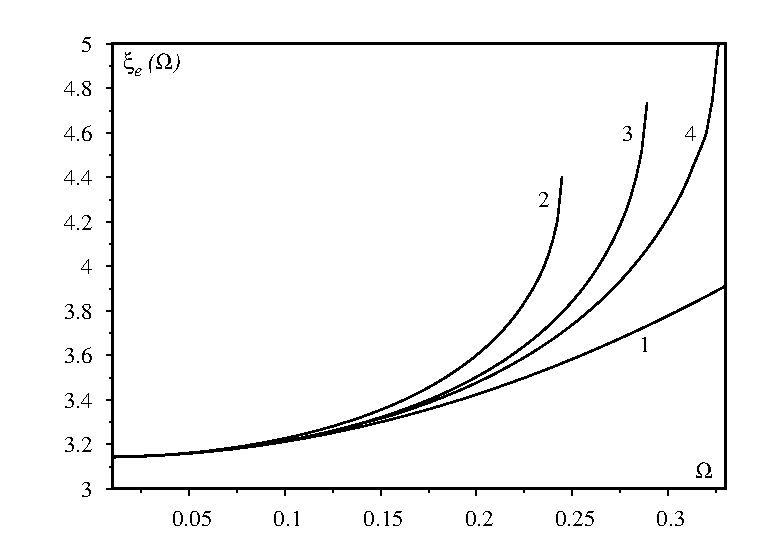
\includegraphics[width=.7\textwidth]{fig_01.eps}
\caption{Dependence of the equatorial radius $\xi_{e}(\Omega)$  on the rotation velocity $\Omega$ for the polytrope with $n=1$ in different approximations. Curve 1 is built on the results of  \citet{1933MNRAS..93..390C}, curve 2 corresponds to our approximation \eqref{eq_036da} at $l_{0}=2$. Curve is 3 built on the results of \citet{1964ApJ...140..552J}, curve 4 -- on the work of \citet{1980Ap&SS..71..415C}.}
\label{fig_01da}
\end{figure}
Dependence of the equatorial radius on the angular velocity in different approximations is illustrated in Fig.~\ref{fig_01da}. Similarly, dependence of the polar radius on the angular velocity in the same approximations is given in Fig.~\ref{fig_02da}.
\begin{figure}[h!]
\center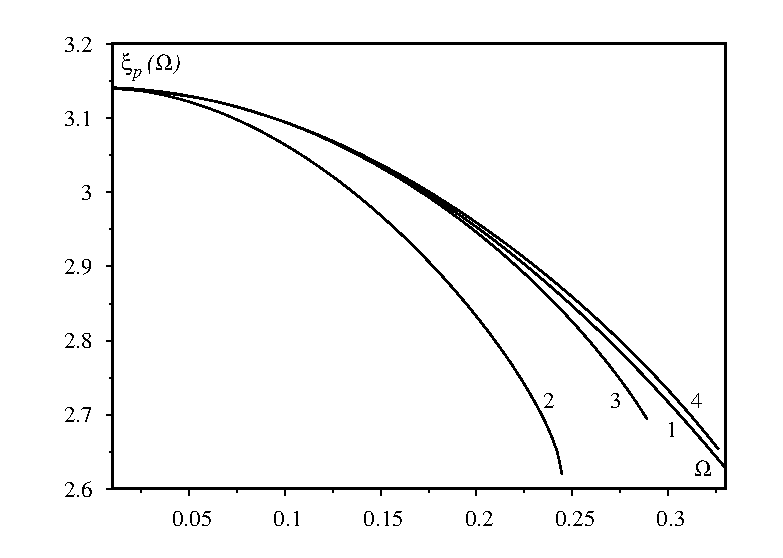
\includegraphics[width=.7\textwidth]{fig_02.eps}
\caption{Dependence of the polar radius $\xi_{p}(\Omega)$  on the rotation velocity $\Omega$ for the polytrope with $n=1$ in different approximations. The notation is the same as in Fig.~\ref{fig_01da}.}
\label{fig_02da}
\end{figure}
As it can be seen from these Figures, the Milne -- Chandrasekhar approximation  is applicable in the vicinity $0\leq\Omega\lesssim 0.5\,\Omega_{\rm max}$, where $\Omega_{\rm max}$=0.2447\ldots. The constants $\alpha_2$ and $\alpha_4$ have the opposite signs and significantly depend on the angular velocity. In the region $0\leq \Omega\leq 0.5\:\Omega_{\rm max}$ the constant $\alpha_4$ is small, and in the region $\Omega > 0.5 \Omega_{\rm max}$ it is close to $|\alpha_2|$. Since in the region $0 \leq\xi\leq\xi_e \:(\Omega_{\rm max})$ the functions $j_2 (\xi)$ and $j_4 (\xi)$ are positive, the approximation $\alpha_4=0$ is only applicable in the region of small velocities $\Omega$.

Approximation \eqref{eq_037da} at $\tilde{l}_0=1$ corresponds to the works of \citet{1933MNRAS..93..390C} and \citet{1980Ap&SS..71..415C}. Herewith, in the work of \citet{1933MNRAS..93..390C} the constant $\alpha_2$  is determined by expression \eqref{eq_045da} at $\xi_1 =\pi$, and in the work of \citet{1980Ap&SS..71..415C} it is calculated numerically based on the calculation of the change of the gravitational potential caused by the rotation. The critical values of the angular velocity given by the authors are: $\Omega_{\rm max} \approx 0.3315$ \citep{1933MNRAS..93..390C} and $\Omega_{\rm max} \approx 0.3264\ldots$ \citep{1980Ap&SS..71..415C}. In fact, the results obtained by the latter author improve the results of \citet{1933MNRAS..93..390C}. The approximation of Milne and Chandrasekhar \citep{1923MNRAS..83..118M,1933MNRAS..93..390C} is also used by \citep*{1965MNRAS.131...13M} for the description of the inner polytrope region, the radius of which is close to the Emden radius. It is found the maximal value of the velocity $\Omega_{\rm max}\approx 0.2755$. In the work of \citet{1964ApJ...140..552J} the polytrope characteristics are calculated numerically. The index $n=1$ corresponds to $\Omega_{\rm max}\cong 0.2891\ldots.$ From these comparisons it follows: the more precise calculation, the smaller value of the critical velocity $\Omega_{\rm max}$.

Given the known coefficients $\alpha_{2l}$, we can build the polytrope surface using Eq.~\eqref{eq_041da}. The meridional polytrope section in approximation \eqref{eq_032da} is shown in Fig.~\ref{fig_03da} for two fixed values of the angular velocity $\Omega_1=0.2$ and $\Omega_2=0.2447$. As it is shown in the Figure, at the angular velocity far from the maximal angular velocity $\Omega_{\rm max}$ the curve 1 coincides with crosses which are built according to \eqref{eq_023da} and \eqref{eq_036da}. However, at the angular velocity $\Omega_{\rm max}$, the real polytrope surface (curve 3) is significantly different from the surface of the auxiliary ellipsoid \eqref{eq_023da}.

\begin{figure}[h!]
\center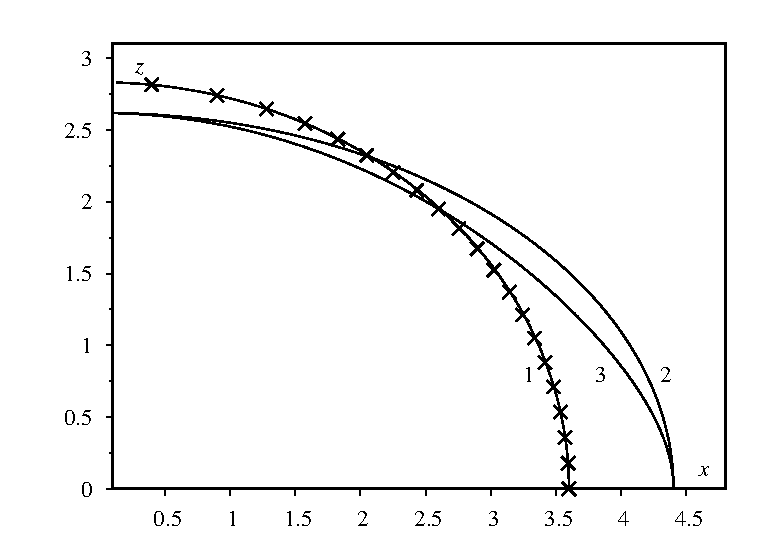
\includegraphics[width=.7\textwidth]{fig_03.eps}
\caption{The meridional section of the polytrope surface. Curve 1 corresponds to formulae \eqref{eq_023da} which determine  the rotational polytrope surface at the angular velocity $\Omega_1=0.2$. Curve 2 -- the same but for $\Omega_2=0.2447$. Curve 3 is built according to formula \eqref{eq_036da} at $\Omega_2=0.2447$. Crosses are built according to formula \eqref{eq_036da} at $\Omega_1=0.2$.}
\label{fig_03da}
\end{figure}

The distribution of matter inside the polytrope determines the gravitational potential outside it
\begin{equation}
\label{eq_049da}
\Phi_{\rm grav}({\bf r})=-G\int\frac{d{\bf r}'\rho_{\rm c}}{|{\bf r}-{\bf r}'|}Y(\xi')=
-\frac{GM}{r}\left\{1-\sum\limits_{l=1}^\infty P_{2l}(\cos\theta)\left(\frac{\lambda}{r}\right)^{2l}J_{2l}(\Omega)\right\},
\end{equation}
where
\begin{equation}
\label{eq_050da}
J_{2l}(\Omega)=-\left\{\int\limits_{-1}^{1}dt'\int\limits_{0}^{\xi_0(t')}d\xi'(\xi')^2Y(\xi',t')\right\}^{-1}
\int\limits_{-1}^{1}dt'P_{2l}(t')\int\limits_{0}^{\xi_0(t')}d\xi'(\xi')^{2l+2}Y(\xi',t'),
\end{equation}
are the universal dimensionless characteristics, which only depend on the angular velocity $\Omega$. Dependence of  coefficients $J_{2l}(\Omega)$ on the angular velocity $\Omega$ at different values $l$ according to Tab.~\ref{tab_01da} is shown in Fig.~\ref{fig_04da}.
\begin{figure}
\center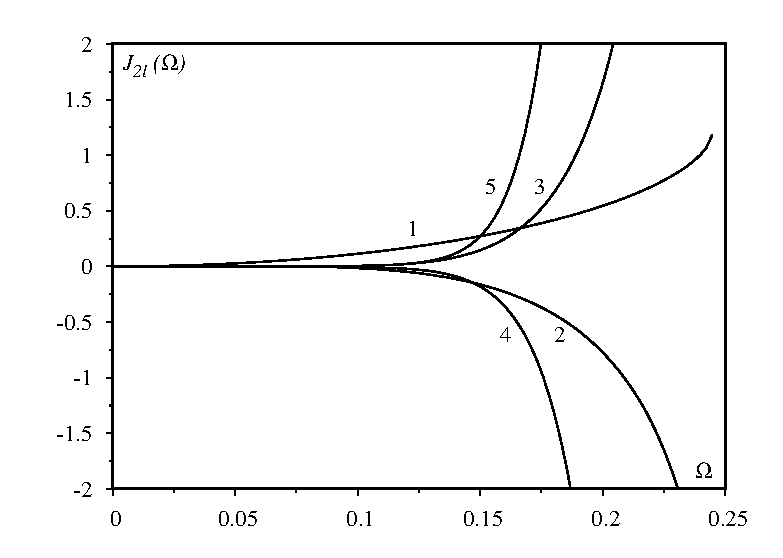
\includegraphics[width=.7\textwidth]{fig_04.eps}
\caption{Dependence of  coefficients (moments of inertia) $J_{2l}(\Omega)$ on the angular velocity $\Omega$  for several values of the parameter $l$ ($1\leq l\leq 5$, $\Delta l=1$) (see Eqs.~\eqref{eq_049da}, \eqref{eq_050da}). Curve 1 corresponds to  $J_{2l}(\Omega)$ at $l=1$, curve 5 -- $l=5$.}
\label{fig_04da}
\end{figure}
At the small angular velocities ($\Omega\leq0.5\,\Omega_{\rm max}$) all coefficients $J_{2l}(\Omega)$ are small values which are proportional to $\Omega^2$.  In this region  coefficient $J_{2}(\Omega)$ is determinative. At the average and rapid angular velocities
($0.5\,\Omega_{\rm max}\leq\Omega\leq\Omega_{\rm max}$)  coefficients $J_{2l}(\Omega)$ strongly depend on the angular velocity $\Omega$. $|J_{2l}(\Omega)|$ is greater for greater $l$.

%________________________________________________________________________________________

\section{The solution of the equilibrium equation at $n=1+\delta$}
\label{sect_06da}

The model of polytrope with $n=1$ is very attractive because in this case we can write the exact solution or its sufficient approximation. However, the polytropic model of a star at $n=1$ is still limited, in a general case the polytrope with axial rotation has four independent parameters $(K,\,\rho_{\rm c},\,\omega\,\text{and}\, n)$, and the equation of state is written in form \eqref{eq_001da}. Because the polytropic model with $n=1$ is a good approximation for massive stars with rapid rotation, it is worth extending it by considering the model with four parameters at $n=1+\delta$, where $\delta$ is a small value.

In the dimensionless form the equilibrium equation is written in the form
\begin{equation}
\label{eq_051da}
\Delta_{\xi,\theta}Y(\xi,\theta)=\Omega^2-Y^{1+\delta}(\xi,\theta),
\end{equation}
and the transition to the dimensionless variables is performed using expressions
\begin{eqnarray}
\label{eq_052da}
\begin{split}
&r=\xi\tilde{\lambda},\,\,\,\rho(r,\theta)=\rho_{\rm c}Y^{1+\delta}(\xi,\theta),\,\,\,
(2+\delta)K=4\pi G\tilde{\lambda}^2\rho_{\rm c}^\gamma,\\
&\gamma=\delta(1+\delta)^{-1},\,\,\,\Omega=\omega(2\pi G\rho_{\rm c})^{-1/2}.
\end{split}
\end{eqnarray}
Analogous to Eq.~\eqref{eq_022da} is now the equation
\begin{equation}
\label{eq_053da}
Y(\xi,\theta)=1+\frac{\Omega^2\xi^2}{6}\:\biggl(1-P_2 (t)\biggr)
+\frac{1}{4\pi}\int Y^{1+\delta}(\xi^{'}, \theta^{'})\:Q ({\boldsymbol\xi},{\boldsymbol\xi}^{'})\:d{\boldsymbol\xi}^{'}.
\end{equation}
It is obvious from the general physical considerations that $\tilde{Y}(\xi,\theta)$ is a monotonous function of the polytropic index. Therefore, at $|\delta|\ll1$ we can use the iteration method in Eq.~\eqref{eq_053da} and in the zero approximation $Y(\xi',\theta')$ is replaced by $Y_1(\xi',\theta')$, which corresponds to $\delta=0$. The first iteration yields
\begin{equation}
\label{eq_054da}
Y(\xi,\theta)=Y_1(\xi',\theta')
+\frac{1}{4\pi}\int\:Q ({\boldsymbol\xi},{\boldsymbol\xi}^{'})\:Y_1(\xi^{'},\theta^{'})[Y_1^{\delta}(\xi^{'}, \theta^{'})-1]\:d{\boldsymbol\xi}^{'}.
\end{equation}
In particular, in the linear approximation over the parameter $\delta$
\begin{equation}
\label{eq_055da}
Y(\xi,\theta)=Y_1(\xi',\theta')
+\frac{\delta}{4\pi}\int\:Q ({\boldsymbol\xi},{\boldsymbol\xi}^{'})\:Y_1(\xi^{'},\theta^{'})\ln Y_1(\xi^{'},\theta^{'})\:d{\boldsymbol\xi}^{'}.
\end{equation}
Expanding the kernel $Q ({\boldsymbol\xi},{\boldsymbol\xi}^{'})$ in series of the Legendre polynomials, we obtain the final representation
\begin{equation}
\label{eq_056da}
Y(\xi,\theta)=Y_1(\xi,\theta)+\frac{\delta}{2}\left\{f_{0}(\xi)+\sum\limits_{l=1}^{\infty}P_{2l}(t)f_{2l}(\xi)\right\}.
\end{equation}
The functions $f_0(\xi)$ and $f_{2l}(\xi)$ are determined by the following expressions:
\begin{eqnarray}
\label{eq_057da}
\begin{split}
& f_{0}(\xi)=-\int\limits_0^{\xi}d\xi'\xi'\int\limits_{-1}^{1}dt'\Psi(\xi',t')+\frac{1}{\xi}\int\limits_0^\xi d\xi'(\xi')^2
\int\limits_{-1}^{1}dt'\Psi(\xi',t'),\\
& f_{2l}(\xi)=(\xi)^{-1-2l}\int\limits_0^\xi d\xi'(\xi')^{2l+2}\int\limits_{-1}^{1}dt'P_{2l}(t')\Psi(\xi',t')+\\
&+\xi^{2l}\int\limits_{-1}^{1}dt'P_{2l}(t')\int\limits_{\xi}^{\xi_0(t')}d\xi'(\xi')^{1-2l}\Psi(\xi',t');\,\,
\Psi(\xi',t')=Y_1(\xi',t')\ln{[Y_1(\xi',t')]}.
\end{split}
\end{eqnarray}
A general solution, $Y(\xi,\theta)$, according to expression \eqref{eq_056da} at a fixed value of the angular velocity $\Omega=0.2$ is shown in Fig.~\ref{fig_05da}. In this case $Y_1(\xi,\theta)$ is determined by expression \eqref{eq_036da}. As it is shown in Figure~\ref{fig_05da} at the positive values $\delta$ we have the increase of both the equatorial and polar radii. This corresponds to the general behavior of the polytrope radius without rotation when varying the index $n$.
\begin{figure}[h!]
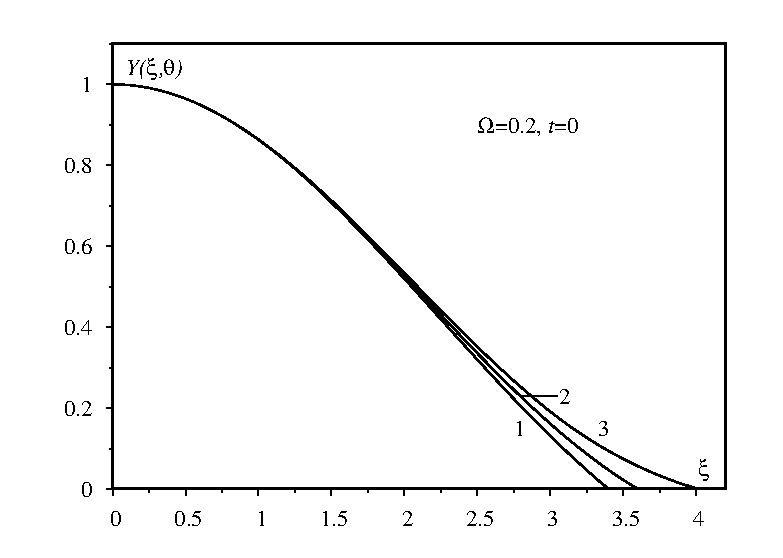
\includegraphics[width=.5\textwidth]{fig_05a.eps}\hfil
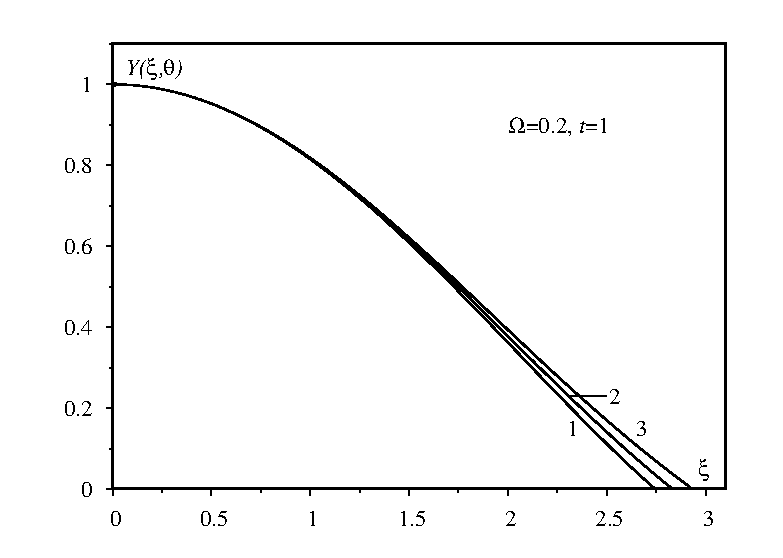
\includegraphics[width=.5\textwidth]{fig_05b.eps}
\caption{A general solution of the equilibrium equation $Y(\xi,\theta)$ according to the expression \eqref{eq_056da} at fixed values $\Omega$ and $t$. Curves 1 correspond to the equilibrium equation at $\delta=-0.1$, curves 2 -- $\delta=0$, curves 3 -- $\delta=0.1$.}
\label{fig_05da}
\end{figure}

%________________________________________________________________________________________

\section{The inverse problem for the polytrope with index $n=1$}
\label{sect_07da}

The polytrope with $n=1$ can be used for the construction of simple polytropic models of stars of early spectral classes, for which significant velocities of angular rotation are typical \citep{2015MNRAS.448..456K}. Such a model has three independent parameters $K,\,\rho_{\rm c},\,\omega$, which have to be determined for the individual observable star. If only the mass $M$ and the equatorial radius $R_e$ are reliably known from observations, then we can only find a narrow variation range for model parameters. For example, we consider the model for the star $\alpha$ Eri ($M=9.7466\cdot10^{30}\,\text{kg}=4.9\,M_\odot,\,R_e=8.3520\cdot10^9\,\text{m}=12\,R_\odot$), the parameters of which are considered in the works of \citet{2015MNRAS.448..456K} and \citet{2017MNRAS.467.4965K}. Taking into account the results of these works, we consider the model in a small variation range of the dimensionless angular velocity $\Omega_0\leq\Omega\leq\Omega_{\rm max}$. Using the results of our calculations from Tables~\ref{tab_01da} and~\ref{tab_02da}, for each $\Omega$ we find the corresponding values $e(\Omega)$ and $\xi_e(\Omega)$. From the relation
\begin{equation}
\label{eq_058da}
\frac{M}{R_e^3}=4\pi^2\eta(\Omega)\rho_{\rm c}\xi_e^{-3}(\Omega)
\end{equation}
we find the density in the stellar centre $\rho_{\rm c}(\Omega)$. From the relation
\begin{equation}
\label{eq_059da}
R_e=\xi_e(\Omega)\left(\frac{K}{2\pi G}\right)^{1/2}
\end{equation}
we determine the parameter $K$, and from definition \eqref{eq_009da} we obtain $\omega(\Omega)$. In the work of \citet{2015MNRAS.448..456K} the angular velocity was not determined, but there was used its value at the stellar equator obtained from observations with the help of the Doppler effect. Such a value of the angular velocity is bigger than the angular velocity in the polytrope model due to the presence of differential rotation.    
For the model with eccentricity $e=0.7454$, which is used by \citet{2015MNRAS.448..456K}, at $\Omega=0.23655$ and the dimensionless equatorial radius $\xi_e(\Omega)=4.02993$ in approximation \eqref{eq_036da}, we obtain 
\begin{equation}
\label{eq_060da}
K_1=1.801\cdot10^9\,\text{Pa\,m}^6\,\text{(kg)}^{-2},\,
\rho_{\rm c}^{(1)}=22.588\,\text{kg\,m}^{-3},\,
\omega_1=2.302\cdot10^{-5}\,\text{s}^{-1}.
\end{equation}
At $\Omega=0.24396$ the dimensionless equatorial radius $\xi_e(\Omega)=4.12304$ in approximation \eqref{eq_037da}, therefore
\begin{equation}
\label{eq_061da}
K_2=1.721\cdot10^9\,\text{Pa\,m}^6\,\text{(kg)}^{-2},\,
\rho_{\rm c}^{(2)}=24.045\,\text{kg\,m}^{-3},\,
\omega_2=2.450\cdot10^{-5}\,\text{s}^{-1}.
\end{equation}
Comparing with the result of \citet{2015MNRAS.448..456K} ($K_0=1.75\cdot10^9\,\text{Pa\,m}^6\,\newline\text{(kg)}^{-2}$), we can see that the parameter $K>K_0$ from approximation \eqref{eq_036da}, and $K<K_0$ from approximation \eqref{eq_037da}.
The approximate solution of the equilibrium equation in the form
\begin{equation}
\label{eq_062da}
\frac{3}{8}Y(\xi,\theta)+\frac{5}{8}\tilde{Y}(\xi,\theta)
\end{equation}
(which is close to the ``gold section''), where $Y(\xi,\theta)$ and $\tilde{Y}(\xi,\theta)$ are determined by expressions \eqref{eq_036da} and \eqref{eq_037da} at $\Omega=0.241496$ and $\xi_e(\Omega)=4.08559$, which is calculated numerically, allows us to determine the polytropic parameters
\begin{equation}
\label{eq_063da}
K=1.752\cdot10^9\,\text{Pa\,m}^6\,\text{(kg)}^{-2},\,
\rho_{\rm c}=23.437\,\text{kg\,m}^{-3},\,
\omega=2.394\cdot10^{-5}\,\text{s}^{-1},
\end{equation}
which almost coincide with those of \citet{2015MNRAS.448..456K}. To simplify the usage of formula \eqref{eq_062da}, we represented  dependencies of the coefficients $\alpha_{2l}$ and $a_{2l}$ as the functions of the angular velocity in the form of Pad\'e approximants. Thereby we obtained the analytical dependence of the equilibrium equation solutions on both the coordinates and $\Omega$. The deviation of the obtained angular velocity calculated by \citet{2015MNRAS.448..456K} from the observed value for $\alpha$ Eri $(2.97\cdot10^{-5}\,\text{s}^{-1})$ we can explain with the differential rotation of the stellar surface layers. Based on the found parameters $K,\,\rho_{\rm c}$ and $\Omega$ we calculated  coefficients $J_{2l}(\Omega)$ for the model of $\alpha$ Eri, which are given in Tab.~\ref{tab_03da}.
\begin{table}[htb]
{\caption{Coefficients $J_{2l}(\Omega)$ for the model of $\alpha$ Eri for different values of~$l$.
\label{tab_03da}}}
\center{
\scalebox{0.9}{
\begin{tabular}{*{6}{c}}
\hline\hline
$l$ & $1$ & $2$ & $3$ & $4$ & $5$\\
\hline
$J_{2l}(\Omega)$ & $0.934751$ & $-2.65689$ & $11.8846$ & $-68.2954$ & $459.572$\\
\hline\hline
\end{tabular}}}
\end{table}
For the comparison with results of  \citet{2015MNRAS.448..456K}, we should replace the length scale $\lambda$ with the scale $R_e=8.3520\cdot10^9\,\text{m}$, writing the potential $\Phi_{\rm grav}({\bf r})$ in the form
\begin{equation}
\label{eq_064da}
\Phi_{\rm grav}({\bf r})=-\frac{GM}{R_e}\frac{1}{\tilde{r}}
\left\{1-\sum\limits_{l=1}^{\infty}\frac{P_{2l}(\cos\theta)}{\tilde{r}^{2l}}I_{2l}(\Omega)\right\},
\end{equation}
where $I_{2l}(\Omega)=J_{2l}(\Omega)\cdot(\lambda/R_e)^{2l},\,\tilde{r}=r/R_e$. Found in this way $I_{2l}(\Omega)$ are close to those of \citet{2015MNRAS.448..456K}. In particular, at $l=1$ we obtain $I_2(\Omega)=0.05603$, which differs from that of \citet{2015MNRAS.448..456K} by less than 2.4\%.

\begin{table}[htb]
\caption{The parameters $K$ and $\rho_c$ of the polytropic model according to the averaged rotational velocities of main-sequence stars.(The observable values $M,\,R,\,\omega$ are taken from the work of~\citet{1965Obs....85..166M}).
\label{tab_04da}}
\center{
\scalebox{0.75}{
\begin{tabular}{*{9}{c}}
\hline\hline
\text{Sp} & $M,\,10^{30}\text{kg}$ & $R,\,10^{9}\text{m}$ & $\omega,\,10^{-5}\text{s}^{-1}$ & $\text{K},\,10^9\text{Pa}\cdot\text{m}^6(\text{kg})^{-2}$ & $\rho_c,\,\text{kg/m}^3$ & $\xi_e(\Omega)$ & $\Omega$ & $\eta(\Omega)$\\
\hline
$\text{O}5$ & $79$ & $12$ & $1.5$ & $5.69709$ & $38.6225$ & $3.25561$ & $0.118$ & $1.03462$\\
$\text{B}0$ & $34$ & $5.3$ & $3.8$ & $1.08767$ & $197.267$ & $3.29082$ & $0.133$ & $1.04508$\\
$\text{B}5$ & $14$ & $2.8$ & $7.6$ & $0.29196$ & $573.682$ & $3.35562$ & $0.155$ & $1.06400$\\
$\text{A}0$ & $7.1$ & $1.8$ & $10.0$ & $0.12207$ & $1081.91$ & $3.33617$ & $0.149$ & $1.05836$\\
$\text{A}5$ & $4.4$ & $1.2$ & $13.0$ & $0.055583$ & $2206.65$ & $3.29602$ & $0.135$ & $1.04661$\\
$\text{F}0$ & $3.5$ & $0.94$ & $10.0$ & $0.036262$ & $3428.6$ & $3.19653$ & $0.084$ & $1.01682$\\
$\text{F}5$ & $2.8$ & $0.84$ & $3.0$ & $0.029897$ & $3720.64$ & $3.14589$ & $0.024$ & $1.00132$\\
$\text{G}0$ & $2.1$ & $0.73$ & $1.6$ & $0.022626$ & $4242.68$ & $3.14266$ & $0.012$ & $1.00033$\\
\hline\hline
\end{tabular}}}
\end{table}

It makes also sense to define approximately the polytropic model parameters for a certain class of stars with rapid rotation. We used the averaged (statistical) values of masses and radii of stars of early spectral classes (O5$\div$G0) from the work of \citet{1965Obs....85..166M}. Taking the radii, which are given in Tab.~\ref{tab_04da} as equatorial, we calculated the values of the parameters $K$ and $\rho_{\rm c}$ in approximation \eqref{eq_062da} for the grid parameters of the values $\varepsilon=R_p/R_e$. From this grid we selected results that correspond to those $\varepsilon$ at which the calculated values $\omega$ coincide with submitted ones in the work of \citet{1965Obs....85..166M}. 
Dependence of the parameters of the ``class'' model $K$ and $\rho_{\rm c}$ on the mass of stars obtained here turned out to be expected: large values of $K$ (small $\rho_{\rm c}$) correspond to massive stars in which the density of matter is small; and small values of $K$ (large $\rho_{\rm c}$) correspond to low-mass stars in which the central density of matter is large. Although the obtained results are approximate, they illustrate dependence of the polytrope parameters on the spectral class or average stellar mass.

\section{Conclusions}
\label{sect_08da}

The polytrope model with $n=1$ takes the central place in the polytropic theory with axial rotation. Due to its simplicity it allows us to obtain the solutions of the equilibrium equation with high precision and yields a reliable values of the model characteristics. Therefore, finding the solution of the equilibrium equation of this model in different approximations and their application is one of actual problems of astrophysics. We obtained a simple analytical shape of the solution of the differential equilibrium Eqs.~\eqref{eq_002da}, \eqref{eq_008da} for the polytrope with $n=1$ and solid-body rotation in the form of infinite series \eqref{eq_032da} or \eqref{eq_034da}. Both variants allow approximations in the form of series with a small number of terms \eqref{eq_036da} and \eqref{eq_037da}, or their linear combinations \eqref{eq_038da}. The practical calculation of the coefficients $\alpha_{2l}$ were performed based on the integral form of  Eq.~\eqref{eq_022da}, that is reduced to the system of linear equations \eqref{eq_042da}. The system of  Eqs.~\eqref{eq_041da}, \eqref{eq_042da} we solved by a two-stage numerical iteration method. The iteration procedure allows us to calculate simultaneously dependence of the coefficients $\alpha_{2l}$, polar and equatorial radii on the dimensionless angular velocity $\Omega$. The approximation of the exact solution, which is obtained explicitly, allows us to calculate dependence of the mass and the moment of inertia on the angular velocity. In an analogous way we find the constants $a_{2l}$, geometrical and physical characteristics of the model as the functions of $\Omega$ in approximation \eqref{eq_037da}. As it can be seen in Figures and Tables 1 and 2, the critical value of the angular velocity $\Omega_{\rm max}$ is smaller than in the work of other authors. Approximation \eqref{eq_036da} is used for the calculation of the gravitational potential outside the polytrope. Expansions \eqref{eq_036da} and \eqref{eq_037da} have good convergence and the increase in the number of series terms leads to insignificant changes of the characteristics only in the vicinity of $\Omega_{\rm max}$. The convergence of series \eqref{eq_036da} and \eqref{eq_037da} is provided by the Bessel functions, which have standard asymptotics at $\xi\rightarrow0$ \citep{1970hmfw.book.....A}. However, it strongly depends on the angular velocity. For example, for the case of the equator from approximation \eqref{eq_037da} the ratio of individual terms of the series can be represented as
\begin{eqnarray*}
\begin{split}
&f_2:f_4:f_6=1.31:0.02:0.002\quad\text{at}\quad\Omega=0.1,\\
&f_2:f_4:f_6=1.53:0.12:0.007\quad\text{at}\quad\Omega=0.2,\\
&f_2:f_4:f_6=1.44:0.64:0.13\quad\,\,\,\text{at}\quad\Omega=\Omega_{\rm max},\\
\end{split}
\end{eqnarray*}   
where $f_{2l}=a_{2l}(\Omega)P_{2l}(0)j_{2l}(\xi_e)$, $(1\leq l\leq3)$. It can be seen that in an almost entire domain of the angular velocity the convergence  is very good, but it worsens in the vicinity of $\Omega_{\rm max}(1)$. Obviously, finding the solutions of the equilibrium equation in the vicinity of $\Omega_{\rm max}$ deserves special attention.
 
With all its advantages the model with $n=1$ is only one of the polytropic models, which can be used for the description of celestial objects. Therefore, it is appropriate to have precise enough solutions of the mechanical equilibrium equation for the model with $n\ne1$. The solution of the equilibrium equation for the case $n=1+\delta$ (where $\delta$ is a small value) was obtained by the method of the perturbation theory. Dependence of the surface shape of such a polytrope on the parameter $\delta$ corresponds to the famous dependence of the polytrope characteristics on the index $n$ \citep{1933MNRAS..93..390C}. This model can be useful for the description of stars with the very rapid angular velocity $(\Omega\geq0.25)$.

The geometrical and physical characteristics of the polytropic models determine not only the solution of the mechanical equilibrium in the dimensionless form, but also the values of the parameters $K,\,\rho_{\rm c},\,\omega$ for the individual celestial bodies. Therefore, the inverse problem of the theory arises -- finding these parameters according to the known solution of the equilibrium equation and observable characteristics of celestial bodies. As an illustration of our approach we considered the problem of the parameters of the polytropic model for the star $\alpha$ Eri and compared them with the results of the work of \citet{2015MNRAS.448..456K}. In approximation \eqref{eq_062da} the value $K=1.752\cdot10^9\,\text{Pa\,m}^6\,\text{(kg)}^{-2}$ obtained by us almost coincides with that of \citet{2015MNRAS.448..456K}. Coefficients $J_{2l}(\Omega)$ are calculated in approximation \eqref{eq_062da}, which are also close to the coefficients of \citet{2015MNRAS.448..456K}. Moreover, for the first time, we considered the problem of the approximate calculation of the parameters $K$ and $\rho_{\rm c}$ for the full subclasses of stars, namely O5$\div$G0, using the observable data from the work of \citet{1965Obs....85..166M}. 

The considered examples indicate that the simple analytical approximations of the solution of the equilibrium equation obtained by us are useful for the description of celestial bodies, in particular to build stellar models with rapid axial rotation.

\bibliography{Polytropes_ed}

\end{document}
\begin{thebibliography}{}
%ADS_ID 1970hmfw.book.....A
\book{Abramowitz, M. and Stegun, I. A.}{1970}{Handbook of mathematical functions: 
		with formulas, graphs, and mathematical tables}{Government Printing Office}{Washington}

%ADS_ID 1980Ap%26SS..71..415C
\article{Caimmi, R.}{1980}{\apss}{71}{415, DOI: 10.1007/BF00639402}

%ADS_ID 1931ApJ....74...81C
\article{Chandrasekhar, S.}{1931}{\apj}{74}{81, DOI: 10.1086/143324}

%ADS_ID 1933MNRAS..93..390C
\article{Chandrasekhar, S.}{1933}{\mnras}{93}{390, DOI: 10.1093/mnras/93.5.390}

%ADS_ID  1969efe..book.....C
\book{Chandrasekhar, S.}{1969}{Ellipsoidal Figures of Equilibrium}{Yale University Press}{New Haven}

%ADS_ID  1926ics..book.....E
\book{Eddington, A.S.}{1926}{The Internal Constitution of the Stars}{Cambridge University Press}{Cambridge}

%ADS_ID  1907gask.book.....E
\book{Emden, R.}{1907}{Gaskugeln}{Leipzig}{Berlin}

%ADS_ID 1930MNRAS..91...63F
\article{Fowler, R.H.}{1930}{\mnras}{91}{63, DOI: 10.1093/mnras/91.1.63}

%ADS_ID 1964ApJ...140..552J
\article{James, R. A.}{1964}{\apj}{140}{552, DOI: 10.1086/147949}

%ADS_ID 2017MNRAS.467.4965K
\article{Knopik, J., Mach, P., Odrzywo\l ek,  A.}{2017}{\mnras}{467}{4965, DOI: 10.1093/mnras/stx164}

%ADS_ID 2015MNRAS.448..456K
\article{Kong, D., Zhang, K., Schubert, G.}{2015}{\mnras}{448}{456, DOI: 10.1093/mnras/stu2759}

%ADS_ID 1937ZA.....14..135K
\article{Kopal, Z.}{1937}{Zeitschrift f\"ur Astrophysik}{14}{135}

%ADS_ID 1870AmJS...50...57L
\article{Lane, J.H.}{1870}{American Journal of Science}{50}{57, DOI: 10.2475/ajs.s2-50.148.57}

%ADS_ID 1965Obs....85..166M
\article{McNally, D.}{1965}{The Observatory}{85}{166}

%ADS_ID 1923MNRAS..83..118M
\article{Milne, E. A.}{1923}{\mnras}{83}{118, DOI: 10.1093/mnras/83.3.118}

%ADS_ID 1965MNRAS.131...13M
\article{Monaghan, J.J., Roxburgh, I.W.}{1965}{\mnras}{131}{13, DOI: 10.1093/mnras/131.1.13}

%ADS_ID 2010JPS.14...4901V
\article{Vavrukh, M.V., Smerechynskyi, S.V., Tyshko, N.L.}{2010}{Journal of Physical Studies}{14}{4901, DOI: 10.30970/jps.14.4901}

%ADS_ID 2019MMC.6...153V
\article{Vavrukh, M.V., Tyshko, N.L., Dzikovskyi, D.V., Stelmakh, O.M.}{2019}{Mathematical Modeling and Computing}{6}
{153, DOI: 10.23939/mmc2019.02.153}  
\end{thebibliography}
                                                                                                             
